\titleformat{\chapter}{}{}{0em}{\bf\LARGE}

Η χρήση του reflection επιτρέπει την επισκόπηση και την τροποποίηση κλάσεων, πεδίων, μεθόδων και κατασκευαστών κατά τον χρόνο εκτέλεσης του προγράμματος.

Μετά την επιτυχή μεταγλώττιση του κώδικα κατασκευάζεται αυτόματα από τον μεταγλωττιστή ένα μπλοκ που ονομάζεται Assembly και περιέχει την ενδιάμεση γλώσσα και μεταδεδομένα.

Τα μεταδεδομένα αποτελούνται από πληροφορίες σχετικά με τις κλάσεις, τις μεθόδους, τους κατασκευαστές κτλ. Με το reflection γίνεται έλεγχος αυτών των μεταδεδομένων για την ανάκτηση πληροφοριών ενός assembly.

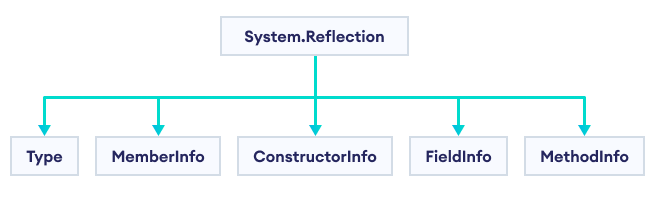
\includegraphics[width=\fullwidthimage]{code/Reflection/csharp-reflection-hierarchy.png}

Η βασική μέθοδος πρόσβασης στα μεταδεδομένα γίνεται με τη χρήση της κλάσης \codebox{Type}, η οποία παρέχει μεθόδους και ιδιότητες που δίνουν πληροφορίες για κάποιον τύπο.

Για παράδειγμα, για τις κλάσεις (\ref{inheritanceClasses}) του παραδείγματος της κληρονομικότητας (\ref{inheritance}), με reflection μπορεί να γίνει εξακρίβωση του τύπου της κάθε μεταβλητής όπως στον κώδικα \ref{reflectionInheritance}.

\begin{listing}[htbp]
\begin{minted}[]{csharp}
Animal dog = new Dog("Max");
Animal cat = new Cat("Dora");

Type type = dog.GetType();
Type type2 = cat.GetType();

Console.WriteLine(type);
Console.WriteLine(type2);
\end{minted}
\caption{Εξακρίβωση τύπου μεταβλητών της κλάσης του κώδικα \ref{inheritanceClasses}}
\label{reflectionInheritance}
\end{listing}

\begin{listing}[htbp]
\begin{minted}[]{csharp}
internal class NoChanging
{
    private string _shouldNotChange;
    public string ShouldNotChange => _shouldNotChange;

    public NoChanging(string shouldNotChange)
    {
        _shouldNotChange = shouldNotChange;
    }
}
\end{minted}
\caption{Κλάσης με private πεδίο και μέθοδο}
\label{reflectionClass}
\end{listing}

Σε άλλο παράδειγμα, για την κλάση του κώδικα \ref{reflectionClass}, μπορεί να γίνει απαρίθμηση των μεθόδων μίας κλάσης, όπως στο παράδειγμα του κώδικα \ref{reflectionProperties}.

\begin{listing}[htbp]
\begin{minted}[]{csharp}
NoChanging a = new NoChanging("First!");

var properties = a.GetType().GetProperties();

Console.WriteLine("Listing class properties...");
foreach (var property in properties)
{
    Console.WriteLine(property.Name, property.PropertyType);
}
\end{minted}
\caption{Απαρίθμηση μεθόδων}
\label{reflectionProperties}
\end{listing}

\newpage
Με reflection μπορούν τα τροποποιηθούν ακόμα και private πεδία μίας κλάσης όπως στο παράδειγμα \ref{reflectionChangePrivate}.

\begin{listing}[htbp]
\begin{minted}[]{csharp}
NoChanging a = new NoChanging("First!");

Console.WriteLine($"Initial value of private " +  
    $"field: {a.ShouldNotChange}");
Console.WriteLine($"Trying to change it...");

var str = a
    .GetType()
    .GetField("_shouldNotChange", 
        BindingFlags.NonPublic | BindingFlags.Instance);

str.SetValue(a, "Second!");

Console.WriteLine($"It changed(!!): {a.ShouldNotChange}");
\end{minted}
\caption{Τροποποίηση private πεδίου}
\label{reflectionChangePrivate}
\end{listing}

